\documentclass{standalone}
\usepackage{tikz}
\usetikzlibrary{patterns, positioning}

\begin{document}
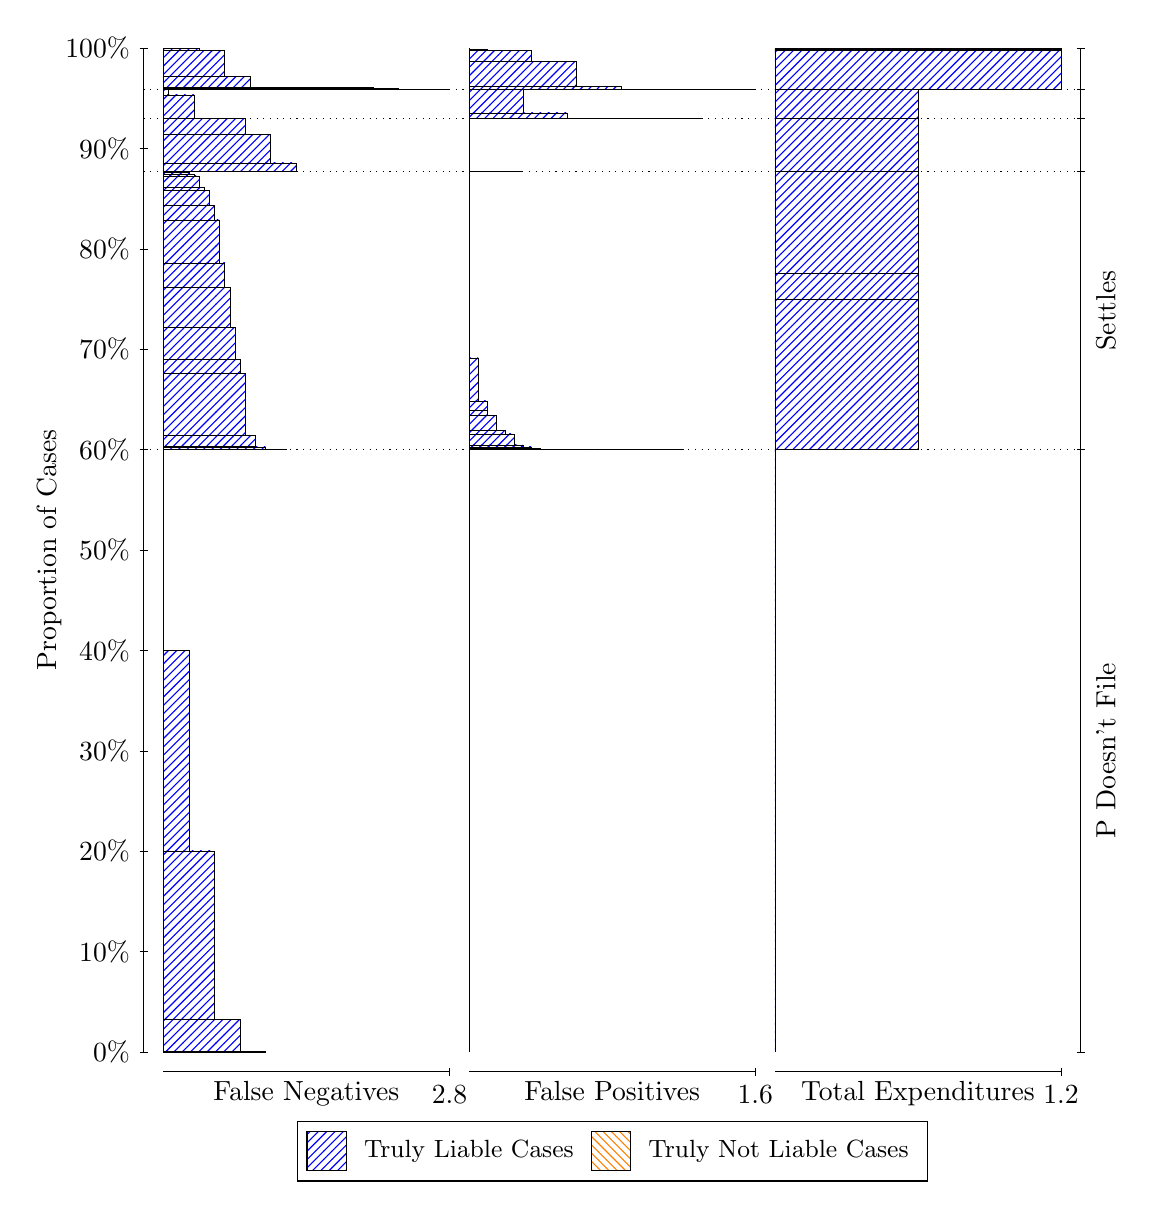
\begin{tikzpicture}
\draw[black, very thin] (1.5,1.75) -- (1.5,14.5);
\node[rotate=90, anchor=center] at (0.3, 8.125) {Proportion of Cases};
\draw[black, very thin] (1.45,1.75) -- (1.55,1.75);
\node[anchor=east] at (1.45, 1.75) {0\%};
\draw[black, very thin] (1.45,3.025) -- (1.55,3.025);
\node[anchor=east] at (1.45, 3.025) {10\%};
\draw[black, very thin] (1.45,4.3) -- (1.55,4.3);
\node[anchor=east] at (1.45, 4.3) {20\%};
\draw[black, very thin] (1.45,5.575) -- (1.55,5.575);
\node[anchor=east] at (1.45, 5.575) {30\%};
\draw[black, very thin] (1.45,6.85) -- (1.55,6.85);
\node[anchor=east] at (1.45, 6.85) {40\%};
\draw[black, very thin] (1.45,8.125) -- (1.55,8.125);
\node[anchor=east] at (1.45, 8.125) {50\%};
\draw[black, very thin] (1.45,9.4) -- (1.55,9.4);
\node[anchor=east] at (1.45, 9.4) {60\%};
\draw[black, very thin] (1.45,10.675) -- (1.55,10.675);
\node[anchor=east] at (1.45, 10.675) {70\%};
\draw[black, very thin] (1.45,11.95) -- (1.55,11.95);
\node[anchor=east] at (1.45, 11.95) {80\%};
\draw[black, very thin] (1.45,13.225) -- (1.55,13.225);
\node[anchor=east] at (1.45, 13.225) {90\%};
\draw[black, very thin] (1.45,14.5) -- (1.55,14.5);
\node[anchor=east] at (1.45, 14.5) {100\%};

\draw[black, very thin] (13.4,1.75) -- (13.4,14.5);
\draw[black, very thin] (13.35,1.75) -- (13.45,1.75);
\node[anchor=west] at (13.35, 1.75) {};
\draw[black, very thin] (13.35,9.4013) -- (13.45,9.4013);
\node[anchor=west] at (13.35, 9.4013) {};
\draw[black, very thin] (13.35,12.935) -- (13.45,12.935);
\node[anchor=west] at (13.35, 12.935) {};
\draw[black, very thin] (13.35,13.605) -- (13.45,13.605);
\node[anchor=west] at (13.35, 13.605) {};
\draw[black, very thin] (13.35,13.978) -- (13.45,13.978);
\node[anchor=west] at (13.35, 13.978) {};
\draw[black, very thin] (13.35,14.5) -- (13.45,14.5);
\node[anchor=west] at (13.35, 14.5) {};

\draw[black, very thin, pattern color=blue, pattern=north east lines] (1.75,1.75) rectangle (3.0476,1.7541);
\draw[black, very thin, pattern color=blue, pattern=north east lines] (1.75,1.7541) rectangle (2.7232,2.1592);
\draw[black, very thin, pattern color=blue, pattern=north east lines] (1.75,2.1592) rectangle (2.3988,4.3047);
\draw[black, very thin, pattern color=blue, pattern=north east lines] (1.75,4.3047) rectangle (2.0744,6.8513);
\draw[black, very thin, pattern color=orange, pattern=north west lines] (1.75,6.8513) rectangle (1.75,6.8513);
\draw[black, very thin, pattern color=blue, pattern=north east lines] (1.75,6.8513) rectangle (1.75,9.4013);
\draw[black, very thin, pattern color=blue, pattern=north east lines] (1.75,9.4013) rectangle (3.3071,9.4021);
\draw[black, very thin, pattern color=blue, pattern=north east lines] (1.75,9.4021) rectangle (3.1774,9.403);
\draw[black, very thin, pattern color=blue, pattern=north east lines] (1.75,9.403) rectangle (3.0476,9.4354);
\draw[black, very thin, pattern color=blue, pattern=north east lines] (1.75,9.4354) rectangle (2.9827,9.4355);
\draw[black, very thin, pattern color=blue, pattern=north east lines] (1.75,9.4355) rectangle (2.9179,9.438);
\draw[black, very thin, pattern color=blue, pattern=north east lines] (1.75,9.438) rectangle (2.9179,9.58);
\draw[black, very thin, pattern color=blue, pattern=north east lines] (1.75,9.58) rectangle (2.853,9.5803);
\draw[black, very thin, pattern color=blue, pattern=north east lines] (1.75,9.5803) rectangle (2.7881,10.373);
\draw[black, very thin, pattern color=blue, pattern=north east lines] (1.75,10.373) rectangle (2.7232,10.544);
\draw[black, very thin, pattern color=blue, pattern=north east lines] (1.75,10.544) rectangle (2.6583,10.957);
\draw[black, very thin, pattern color=blue, pattern=north east lines] (1.75,10.957) rectangle (2.5935,10.957);
\draw[black, very thin, pattern color=blue, pattern=north east lines] (1.75,10.957) rectangle (2.5935,11.458);
\draw[black, very thin, pattern color=blue, pattern=north east lines] (1.75,11.458) rectangle (2.5286,11.771);
\draw[black, very thin, pattern color=blue, pattern=north east lines] (1.75,11.771) rectangle (2.5286,11.771);
\draw[black, very thin, pattern color=blue, pattern=north east lines] (1.75,11.771) rectangle (2.4637,12.318);
\draw[black, very thin, pattern color=blue, pattern=north east lines] (1.75,12.318) rectangle (2.3988,12.497);
\draw[black, very thin, pattern color=blue, pattern=north east lines] (1.75,12.497) rectangle (2.3339,12.694);
\draw[black, very thin, pattern color=blue, pattern=north east lines] (1.75,12.694) rectangle (2.3339,12.694);
\draw[black, very thin, pattern color=blue, pattern=north east lines] (1.75,12.694) rectangle (2.269,12.694);
\draw[black, very thin, pattern color=blue, pattern=north east lines] (1.75,12.694) rectangle (2.269,12.735);
\draw[black, very thin, pattern color=blue, pattern=north east lines] (1.75,12.735) rectangle (2.269,12.735);
\draw[black, very thin, pattern color=blue, pattern=north east lines] (1.75,12.735) rectangle (2.2042,12.875);
\draw[black, very thin, pattern color=blue, pattern=north east lines] (1.75,12.875) rectangle (2.2042,12.875);
\draw[black, very thin, pattern color=blue, pattern=north east lines] (1.75,12.875) rectangle (2.1393,12.901);
\draw[black, very thin, pattern color=blue, pattern=north east lines] (1.75,12.901) rectangle (2.0744,12.923);
\draw[black, very thin, pattern color=blue, pattern=north east lines] (1.75,12.923) rectangle (2.0095,12.929);
\draw[black, very thin, pattern color=blue, pattern=north east lines] (1.75,12.929) rectangle (2.0095,12.929);
\draw[black, very thin, pattern color=blue, pattern=north east lines] (1.75,12.929) rectangle (1.9446,12.929);
\draw[black, very thin, pattern color=blue, pattern=north east lines] (1.75,12.929) rectangle (1.9446,12.929);
\draw[black, very thin, pattern color=blue, pattern=north east lines] (1.75,12.929) rectangle (1.9446,12.929);
\draw[black, very thin, pattern color=blue, pattern=north east lines] (1.75,12.929) rectangle (1.8798,12.934);
\draw[black, very thin, pattern color=blue, pattern=north east lines] (1.75,12.934) rectangle (1.8798,12.934);
\draw[black, very thin, pattern color=blue, pattern=north east lines] (1.75,12.934) rectangle (1.8149,12.934);
\draw[black, very thin, pattern color=orange, pattern=north west lines] (1.75,12.934) rectangle (1.75,12.934);
\draw[black, very thin, pattern color=blue, pattern=north east lines] (1.75,12.934) rectangle (1.75,12.935);
\draw[black, very thin, pattern color=blue, pattern=north east lines] (1.75,12.935) rectangle (3.4369,13.04);
\draw[black, very thin, pattern color=blue, pattern=north east lines] (1.75,13.04) rectangle (3.1125,13.407);
\draw[black, very thin, pattern color=blue, pattern=north east lines] (1.75,13.407) rectangle (2.7881,13.602);
\draw[black, very thin, pattern color=blue, pattern=north east lines] (1.75,13.602) rectangle (2.4637,13.605);
\draw[black, very thin, pattern color=blue, pattern=north east lines] (1.75,13.605) rectangle (2.1393,13.605);
\draw[black, very thin, pattern color=orange, pattern=north west lines] (1.75,13.605) rectangle (1.75,13.605);
\draw[black, very thin, pattern color=blue, pattern=north east lines] (1.75,13.605) rectangle (2.1393,13.906);
\draw[black, very thin, pattern color=blue, pattern=north east lines] (1.75,13.906) rectangle (1.8149,13.976);
\draw[black, very thin, pattern color=orange, pattern=north west lines] (1.75,13.976) rectangle (1.75,13.976);
\draw[black, very thin, pattern color=blue, pattern=north east lines] (1.75,13.976) rectangle (1.75,13.978);
\draw[black, very thin, pattern color=blue, pattern=north east lines] (1.75,13.978) rectangle (5.3833,13.978);
\draw[black, very thin, pattern color=blue, pattern=north east lines] (1.75,13.978) rectangle (5.0589,13.978);
\draw[black, very thin, pattern color=blue, pattern=north east lines] (1.75,13.978) rectangle (4.7345,13.987);
\draw[black, very thin, pattern color=blue, pattern=north east lines] (1.75,13.987) rectangle (4.4101,13.998);
\draw[black, very thin, pattern color=blue, pattern=north east lines] (1.75,13.998) rectangle (4.0857,13.999);
\draw[black, very thin, pattern color=blue, pattern=north east lines] (1.75,13.999) rectangle (3.7613,13.999);
\draw[black, very thin, pattern color=blue, pattern=north east lines] (1.75,13.999) rectangle (3.5018,13.999);
\draw[black, very thin, pattern color=blue, pattern=north east lines] (1.75,13.999) rectangle (3.4369,13.999);
\draw[black, very thin, pattern color=blue, pattern=north east lines] (1.75,13.999) rectangle (3.1774,14.005);
\draw[black, very thin, pattern color=blue, pattern=north east lines] (1.75,14.005) rectangle (2.853,14.143);
\draw[black, very thin, pattern color=blue, pattern=north east lines] (1.75,14.143) rectangle (2.5286,14.466);
\draw[black, very thin, pattern color=blue, pattern=north east lines] (1.75,14.466) rectangle (2.2042,14.5);
\draw[black, very thin, pattern color=blue, pattern=north east lines] (1.75,14.5) rectangle (1.8798,14.5);
\draw[black, very thin, pattern color=orange, pattern=north west lines] (1.75,14.5) rectangle (1.75,14.5);
\draw[black, very thin, pattern color=blue, pattern=north east lines] (1.75,14.5) rectangle (1.75,14.5);
\draw[black, very thin, pattern color=orange, pattern=north west lines] (5.6333,1.75) rectangle (5.6333,1.75);
\draw[black, very thin, pattern color=blue, pattern=north east lines] (5.6333,1.75) rectangle (5.6333,9.4013);
\draw[black, very thin, pattern color=orange, pattern=north west lines] (5.6333,9.4013) rectangle (8.3583,9.4013);
\draw[black, very thin, pattern color=blue, pattern=north east lines] (5.6333,9.4013) rectangle (8.3583,9.4013);
\draw[black, very thin, pattern color=orange, pattern=north west lines] (5.6333,9.4013) rectangle (8.1313,9.4013);
\draw[black, very thin, pattern color=blue, pattern=north east lines] (5.6333,9.4013) rectangle (8.1313,9.4013);
\draw[black, very thin, pattern color=orange, pattern=north west lines] (5.6333,9.4013) rectangle (7.9042,9.4013);
\draw[black, very thin, pattern color=blue, pattern=north east lines] (5.6333,9.4013) rectangle (7.9042,9.4013);
\draw[black, very thin, pattern color=blue, pattern=north east lines] (5.6333,9.4013) rectangle (7.7906,9.4013);
\draw[black, very thin, pattern color=orange, pattern=north west lines] (5.6333,9.4013) rectangle (7.6771,9.4013);
\draw[black, very thin, pattern color=blue, pattern=north east lines] (5.6333,9.4013) rectangle (7.6771,9.4013);
\draw[black, very thin, pattern color=blue, pattern=north east lines] (5.6333,9.4013) rectangle (7.5635,9.4013);
\draw[black, very thin, pattern color=orange, pattern=north west lines] (5.6333,9.4013) rectangle (7.45,9.4013);
\draw[black, very thin, pattern color=blue, pattern=north east lines] (5.6333,9.4013) rectangle (7.45,9.4013);
\draw[black, very thin, pattern color=blue, pattern=north east lines] (5.6333,9.4013) rectangle (7.3365,9.4013);
\draw[black, very thin, pattern color=orange, pattern=north west lines] (5.6333,9.4013) rectangle (7.2229,9.4013);
\draw[black, very thin, pattern color=blue, pattern=north east lines] (5.6333,9.4013) rectangle (7.2229,9.4013);
\draw[black, very thin, pattern color=blue, pattern=north east lines] (5.6333,9.4013) rectangle (7.1094,9.4013);
\draw[black, very thin, pattern color=blue, pattern=north east lines] (5.6333,9.4013) rectangle (6.9958,9.402);
\draw[black, very thin, pattern color=orange, pattern=north west lines] (5.6333,9.402) rectangle (6.9958,9.402);
\draw[black, very thin, pattern color=blue, pattern=north east lines] (5.6333,9.402) rectangle (6.9958,9.402);
\draw[black, very thin, pattern color=blue, pattern=north east lines] (5.6333,9.402) rectangle (6.8823,9.4021);
\draw[black, very thin, pattern color=orange, pattern=north west lines] (5.6333,9.4021) rectangle (6.7687,9.4021);
\draw[black, very thin, pattern color=blue, pattern=north east lines] (5.6333,9.4021) rectangle (6.7687,9.4067);
\draw[black, very thin, pattern color=blue, pattern=north east lines] (5.6333,9.4067) rectangle (6.6552,9.4068);
\draw[black, very thin, pattern color=orange, pattern=north west lines] (5.6333,9.4068) rectangle (6.5417,9.4068);
\draw[black, very thin, pattern color=blue, pattern=north east lines] (5.6333,9.4068) rectangle (6.5417,9.4068);
\draw[black, very thin, pattern color=blue, pattern=north east lines] (5.6333,9.4068) rectangle (6.5417,9.4132);
\draw[black, very thin, pattern color=blue, pattern=north east lines] (5.6333,9.4132) rectangle (6.4281,9.4347);
\draw[black, very thin, pattern color=blue, pattern=north east lines] (5.6333,9.4347) rectangle (6.4281,9.4349);
\draw[black, very thin, pattern color=blue, pattern=north east lines] (5.6333,9.4349) rectangle (6.3146,9.4603);
\draw[black, very thin, pattern color=blue, pattern=north east lines] (5.6333,9.4603) rectangle (6.201,9.6005);
\draw[black, very thin, pattern color=blue, pattern=north east lines] (5.6333,9.6005) rectangle (6.0875,9.6415);
\draw[black, very thin, pattern color=blue, pattern=north east lines] (5.6333,9.6415) rectangle (5.974,9.6415);
\draw[black, very thin, pattern color=blue, pattern=north east lines] (5.6333,9.6415) rectangle (5.974,9.8392);
\draw[black, very thin, pattern color=blue, pattern=north east lines] (5.6333,9.8392) rectangle (5.8604,9.9004);
\draw[black, very thin, pattern color=blue, pattern=north east lines] (5.6333,9.9004) rectangle (5.8604,10.018);
\draw[black, very thin, pattern color=blue, pattern=north east lines] (5.6333,10.018) rectangle (5.7469,10.565);
\draw[black, very thin, pattern color=blue, pattern=north east lines] (5.6333,10.565) rectangle (5.6333,12.935);
\draw[black, very thin, pattern color=orange, pattern=north west lines] (5.6333,12.935) rectangle (6.3146,12.935);
\draw[black, very thin, pattern color=blue, pattern=north east lines] (5.6333,12.935) rectangle (6.3146,12.935);
\draw[black, very thin, pattern color=blue, pattern=north east lines] (5.6333,12.935) rectangle (5.7469,12.937);
\draw[black, very thin, pattern color=blue, pattern=north east lines] (5.6333,12.937) rectangle (5.6333,13.605);
\draw[black, very thin, pattern color=orange, pattern=north west lines] (5.6333,13.605) rectangle (8.5854,13.605);
\draw[black, very thin, pattern color=blue, pattern=north east lines] (5.6333,13.605) rectangle (8.5854,13.605);
\draw[black, very thin, pattern color=blue, pattern=north east lines] (5.6333,13.605) rectangle (8.0177,13.605);
\draw[black, very thin, pattern color=blue, pattern=north east lines] (5.6333,13.605) rectangle (7.45,13.607);
\draw[black, very thin, pattern color=blue, pattern=north east lines] (5.6333,13.607) rectangle (6.8823,13.677);
\draw[black, very thin, pattern color=blue, pattern=north east lines] (5.6333,13.677) rectangle (6.3146,13.978);
\draw[black, very thin, pattern color=orange, pattern=north west lines] (5.6333,13.978) rectangle (9.2667,13.978);
\draw[black, very thin, pattern color=blue, pattern=north east lines] (5.6333,13.978) rectangle (9.2667,13.978);
\draw[black, very thin, pattern color=orange, pattern=north west lines] (5.6333,13.978) rectangle (8.699,13.978);
\draw[black, very thin, pattern color=blue, pattern=north east lines] (5.6333,13.978) rectangle (8.699,13.978);
\draw[black, very thin, pattern color=orange, pattern=north west lines] (5.6333,13.978) rectangle (8.1313,13.978);
\draw[black, very thin, pattern color=blue, pattern=north east lines] (5.6333,13.978) rectangle (8.1313,13.978);
\draw[black, very thin, pattern color=blue, pattern=north east lines] (5.6333,13.978) rectangle (7.5635,14.012);
\draw[black, very thin, pattern color=orange, pattern=north west lines] (5.6333,14.012) rectangle (7.5635,14.012);
\draw[black, very thin, pattern color=blue, pattern=north east lines] (5.6333,14.012) rectangle (7.5635,14.012);
\draw[black, very thin, pattern color=blue, pattern=north east lines] (5.6333,14.012) rectangle (6.9958,14.335);
\draw[black, very thin, pattern color=blue, pattern=north east lines] (5.6333,14.335) rectangle (6.9958,14.335);
\draw[black, very thin, pattern color=blue, pattern=north east lines] (5.6333,14.335) rectangle (6.4281,14.471);
\draw[black, very thin, pattern color=blue, pattern=north east lines] (5.6333,14.471) rectangle (6.4281,14.473);
\draw[black, very thin, pattern color=blue, pattern=north east lines] (5.6333,14.473) rectangle (5.8604,14.479);
\draw[black, very thin, pattern color=blue, pattern=north east lines] (5.6333,14.479) rectangle (5.8604,14.479);
\draw[black, very thin, pattern color=orange, pattern=north west lines] (5.6333,14.479) rectangle (5.6333,14.479);
\draw[black, very thin, pattern color=blue, pattern=north east lines] (5.6333,14.479) rectangle (5.6333,14.5);
\draw[black, very thin, pattern color=orange, pattern=north west lines] (9.5167,1.75) rectangle (9.5167,1.75);
\draw[black, very thin, pattern color=blue, pattern=north east lines] (9.5167,1.75) rectangle (9.5167,9.4013);
\draw[black, very thin, pattern color=orange, pattern=north west lines] (9.5167,9.4013) rectangle (11.333,9.4013);
\draw[black, very thin, pattern color=blue, pattern=north east lines] (9.5167,9.4013) rectangle (11.333,11.308);
\draw[black, very thin, pattern color=orange, pattern=north west lines] (9.5167,11.308) rectangle (11.333,11.308);
\draw[black, very thin, pattern color=blue, pattern=north east lines] (9.5167,11.308) rectangle (11.333,11.634);
\draw[black, very thin, pattern color=orange, pattern=north west lines] (9.5167,11.634) rectangle (11.333,11.634);
\draw[black, very thin, pattern color=blue, pattern=north east lines] (9.5167,11.634) rectangle (11.333,12.935);
\draw[black, very thin, pattern color=orange, pattern=north west lines] (9.5167,12.935) rectangle (11.333,12.935);
\draw[black, very thin, pattern color=blue, pattern=north east lines] (9.5167,12.935) rectangle (11.333,13.605);
\draw[black, very thin, pattern color=orange, pattern=north west lines] (9.5167,13.605) rectangle (11.333,13.605);
\draw[black, very thin, pattern color=blue, pattern=north east lines] (9.5167,13.605) rectangle (11.333,13.978);
\draw[black, very thin, pattern color=orange, pattern=north west lines] (9.5167,13.978) rectangle (13.15,13.978);
\draw[black, very thin, pattern color=blue, pattern=north east lines] (9.5167,13.978) rectangle (13.15,14.476);
\draw[black, very thin, pattern color=orange, pattern=north west lines] (9.5167,14.476) rectangle (13.15,14.476);
\draw[black, very thin, pattern color=blue, pattern=north east lines] (9.5167,14.476) rectangle (13.15,14.479);
\draw[black, very thin, pattern color=orange, pattern=north west lines] (9.5167,14.479) rectangle (13.15,14.479);
\draw[black, very thin, pattern color=blue, pattern=north east lines] (9.5167,14.479) rectangle (13.15,14.5);
\draw[black, dotted] (1.5,9.4013) -- (13.4,9.4013);
\draw[black, dotted] (1.5,12.935) -- (13.4,12.935);
\draw[black, dotted] (1.5,13.605) -- (13.4,13.605);
\draw[black, dotted] (1.5,13.978) -- (13.4,13.978);
\draw[black, very thin] (1.75,1.5) -- (5.3833,1.5);
\node[anchor=north] at (3.5667, 1.5) {False Negatives};
\draw[black, very thin] (5.3833,1.45) -- (5.3833,1.55);
\node[anchor=north] at (5.3833, 1.45) {2.8};

\draw[black, very thin] (5.6333,1.5) -- (9.2667,1.5);
\node[anchor=north] at (7.45, 1.5) {False Positives};
\draw[black, very thin] (9.2667,1.45) -- (9.2667,1.55);
\node[anchor=north] at (9.2667, 1.45) {1.6};

\draw[black, very thin] (9.5167,1.5) -- (13.15,1.5);
\node[anchor=north] at (11.333, 1.5) {Total Expenditures};
\draw[black, very thin] (13.15,1.45) -- (13.15,1.55);
\node[anchor=north] at (13.15, 1.45) {1.2};

\node[black, centered, rotate=90] at (13.72, 5.5756) {P Doesn't File};
\node[black, centered, rotate=90] at (13.72, 11.168) {Settles};




\draw (7.449999999999999,1.5) node[draw=none] (baseCoordinate) {};
\begin{scope}[align=center]
        \matrix[scale=0.5, draw=black, below=0.5cm of baseCoordinate, nodes={draw}, column sep=0.1cm]{
            \node[rectangle, draw, minimum width=0.5cm, minimum height=0.5cm, pattern=north east lines, pattern color=blue] {}; &
            \node[draw=none, font=\small] (B) {Truly Liable Cases}; &
            \node[rectangle, draw, minimum width=0.5cm, minimum height=0.5cm, pattern=north west lines, pattern color=orange] {}; &
            \node[draw=none, font=\small] (B) {Truly Not Liable Cases}; \\
            };
\end{scope}

\end{tikzpicture}
\end{document}